% !TeX root = ../thuthesis-example.tex

\chapter{相关研究综述}
本节首先介绍目前主流时序数据库的写入方式,然后介绍与数据库客户端以及 RPC 优化有关的工作。
\section{时序数据库数据写入接口概述}
目前市面上流行的时序数据库有四种常见的数据写入方式:通过 SQL 语句写入、原生接口写入、行协议写入以及通过数据通信协议写入。下面将分别介绍这四种写入方式的细节。
\subsection{通过 SQL 语句写入}
SQL 写入就是通过 SQL 语句进行写入,根据写入数据数据量的不同,又可以分为单表单行写入、单表多行写入和多表写入。应用需要将写入数据的元数据以及数据本体记录到 SQL 文本中,再通过 JDBC、ODBC 或者数据库的客户端将 SQL 语句发送到服务器。具有这一类写入方式的时序数据库有 Apache IoTDB、InfluxDB、TDEngine 等,目前 Apache IoTDB 支持单表单行写入和单表多行写入,InfluxDB 和 TDEngine 则支持单表单行写入、单表多行写入和多表写入。

对于用户而言,使用 SQL 写入最符合直觉。SQL 也是用户和几乎所有数据库交互的一种通用方式。从开发者的角度来说,SQL 是一种和编程语言无关的交互协议,在为数据库开发不同编程语言下的客户端时,使用 SQL 进行写入可以避免对不同编程语言下数据结构的适配,减少开发时的工作量,提高开发效率。

然而,SQL 语句本身是一种文本,服务器在接收到 SQL 语句以后需要通过词法解析、语法解析等流程从 SQL 语句中提取出有效的信息,才能进行下一步的写入操作。而对 SQL 语句的解析需要消耗较多的系统资源,因此从资源利用的角度来说并不高效。因此,Apache IoTDB 在官方文档中明确推荐用户使用原生写入接口以提高写入性能\cite{iotdb2024javanative},InfluxDB 也在其官方教程中推荐用户使用行协议写入以提高性能\cite{influx2024highperformance}。TDEngine 将 SQL 写入作为推荐用户使用的写入方式之一,但是为了避免 SQL 语句解析对服务器资源的挤占,写入 SQL 语句会先在 TDEngine 的客户端进行解析,只有解析出来的结果才会发送到服务器。此外,从功能性的角度来说,SQL 语句只能传递数值类型、布尔类型和文本类型的数据,对于时序场景有可能存在的字节流数据、图片数据等非结构化数据并不友好。
\subsection{原生接口写入}
这种写入方式通过特定的数据结构而不是 SQL 文本来传输需要写入的数据。相比于通过 SQL 语句写入,原生接口写入将更多的信息直接传递给了服务器,不需要服务器从 SQL 语句中提取有效的信息。然而,不同进程之间的数据结构不能直接传输,一般需要在客户端先序列化成二进制数据经过网络进行传输,服务器接收到二进制数据之后再反序列化为原本的数据结构,然后执行后续的写入步骤。

Apache IoTDB 提供了 InsertTablet 和 InsertRecords 两类同步原生写入接口,上层应用分别以 Tablet 和 Records 两种数据结构将数据传递给 SDK,然后 SDK 会将数据交由 Apache Thrift\cite{apache2024thrift} 序列化以后传输到服务器。Apache HoraeDB 提供了 Point 写入接口,每个数据点封装成 Point 的形式,然后一批数据点组成一个 Point 列表传递给写入 SDK。SDK 接收到 Point 列表以后会进行一系列的校验工作,然后使用 ProtocolBuffer\cite{currier2022protocol} 将数据序列化后传输到服务器。

使用原生接口写入的好处是将信息直接以数据结构的形式传递给服务器,服务器无需从 SQL 文本中推测数据的信息。在将数据结构序列化为二进制数据时,也可以根据数据类型的不同进行压缩和编码等优化,减少需要传输的数据量。SQL 等文本协议虽然也可以进行压缩,但是这些协议缺少了对数据类型、数据分布的先验知识,完全把数据当作文本进行压缩,因此效果不如原生接口写入。从这个角度看,原生接口写入在性能上具有天然的优势。王晨等人的工作也表明,Apache IoTDB 在使用 InsertTablet 接口时不仅写入延迟显著低于使用行协议写入的 InfluxDB,写入吞吐也要显著高于 InfluxDB\cite{wang2023apache}。此外,从功能性上来看,原生接口写入不仅可以方便地传递数值、文本和布尔类型的数据,对于字节流或者图片等结构化数据也有较好地支持。例如,IoTDB 的某用户使用 InsertRecords 接口存储卫星发射观测过程中所产生的原始信号数据,如果使用文本类型的协议则无法很好地描述此类数据。

然而,原生接口写入也具有一些缺点。用户在使用原生接口写入时,往往需要了解写入 SDK 对数据结构的定义,然后将数据转换为 SDK 所需的数据结构,这样对用户的开发过程带来了一些负担。其次,对于开发者来说,不同编程语言的数据结构之间有较大的差别,因此需要为不同编程语言下的客户端开发不同的 SDK,这增加了开发者的工作量,也更容易产生软件缺陷。

\subsection{行协议写入}
行协议(Line Protocol)\cite{influx2024lineprotocol}是一种基于文本的写入协议,其中规定了数据写入的格式。例如 InfluxDB 所采用的 InfluxDB 行协议格式为\emph{measureable,metadata1,metadata2 <specific\_field>=<value>}。常见的行协议有 InfluxDB 行协议、OpenTSDB 行协议、Prometheus 行协议等。使用这一类行协议进行写入的数据库有 InfluxDB、OpenTSDB、TDEngine 等。

从本质上来说,行协议与 SQL 类似,都将需要写入的数据格式化到文本中,所以理论上行协议只是一种时序数据领域方言化的广义 SQL。行协议是针对时序数据写入而设计的,一方面其在格式上相比 SQL 更加简洁,在解析过程中的开销相对较小;另一方面其能更加方便地描述时序数据的标签(Tag)、字段(Field)等信息,对于时序数据的特点有更好的支持。在 InfluxDB 的官方文档中提到,使用行协议写入具有如下优点:
\begin{enumerate}
  \item 通过网络传输的数据量更小,可以提高性能和节省成本;
  \item 数据更加易于访问,可以更加方便地进行数据分析;
  \item 磁盘写入更快,行协议的设计支持更高效的磁盘写入操作。
\end{enumerate}
此外,使用行协议进行数据写入也具有与 SQL 类似的通用性,不同编程语言 SDK 的开发工作量也相对较小。

使用行协议的具有以下几个缺点。首先,相较于原生接口写入,行协议仍然要求服务器从文本中提取出写入所需要的信息,这一过程会带来一定的开销。其次,行协议是一种文本协议,对于字节流、图片等非结构化数据的写入并不友好。最后,用户在使用行协议写入时需要一定的学习成本,因为其并不如 SQL 语言那样直观。为了解决最后一个缺点,InfluxDB 等数据库推出了一些客户端工具,如 Telegraf\cite{influx2024telegraf},这些工具对行协议进行了封装,让用户可以以更加直观的方式进行写入。

\subsection{通过数据通信协议写入}
在这种写入方式中,客户端将数据通过常见的数据通信协议进行打包和发送,服务器接收到数据后进行包解析和写入。在物联网场景中,常见的数据通信方式有 OPC 协议\cite{zheng2002opc}、MQTT 协议\cite{soni2017survey}、RESTful API 协议\cite{fielding2000architectural} 等。

OPC 协议的全称为 OLE for Process Control,是一种工业通信标准,旨在促进不同制造商的自动化设备、系统和软件之间的数据交换和互操作性。OPC 标准由 OPC Foundation 维护,该组织由多个硬件制造商、软件开发商和系统集成商组成,共同推动和支持这一开放的、独立于平台的通信标准。OPC 有多个版本,其中 OPC UA(Univerised Architecture)是最新的 OPC 通信标准,具有跨平台、加密安全、按需访问等特性\cite{hannelius2008roadmap},图 \ref{fig:opc-arch} 展示了 OPC 通讯协议的架构图。 在 OPC UA 协议中存在一个 OPC UA Server 的角色,它提供订阅功能,负责进行数据的交换。时序数据库可以向 OPC UA Server 订阅需要写入的时间序列,数据产生后先从客户端上被发往 OPC UA Server,OPC UA Server 再将接收到的数据发送到时序数据库。
\begin{figure}
  \centering
  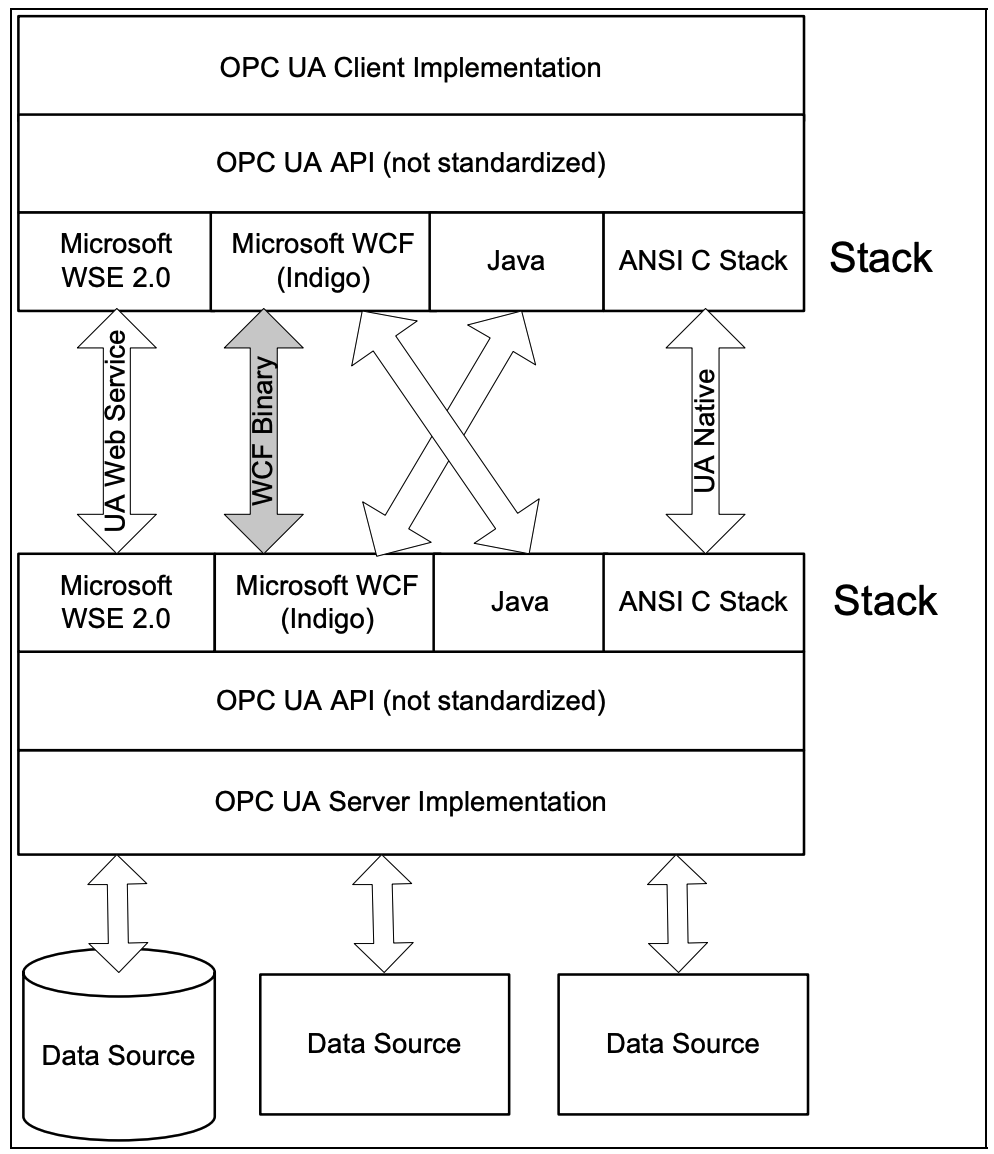
\includegraphics[width=0.7\textwidth]{OPC-UA-arch.png}
  \caption{OPC UA 通讯架构图\cite{leitner2006opc}}
  \label{fig:opc-arch}
\end{figure}


MQTT 协议的全称为 Message Queuing Telemetry Transport,是一种轻量级的、基于发布/订阅模型的消息传输协议,它专为低带宽、高延迟或不可靠的网络环境设计。MQTT 协议因其设计简洁、占用资源少、通信效率高而广泛应用于物联网、移动应用程序、车载系统和智能家居等场景\cite{yassein2017internet}。图 \ref{fig:mqtt-arch} 展示了使用 MQTT 通讯时的架构图。当数据使用 MQTT 协议写入时,客户端将采集到的数据发送到 MQTT 服务器,MQTT 服务器再将数据发送到对应的订阅者,时序数据库可以作为订阅者接收到数据后进行写入。
\begin{figure}
  \centering
  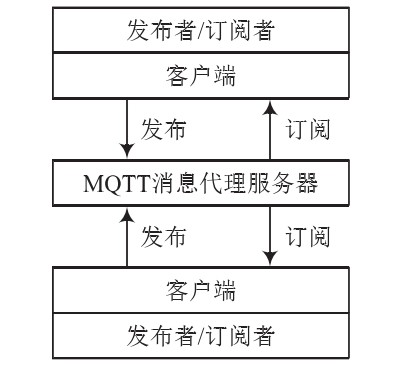
\includegraphics[width=0.4\textwidth]{MQTT-architecture.jpg}
  \caption{MQTT 通讯架构图\cite{WLWJ202404039}}
  \label{fig:mqtt-arch}
\end{figure}

RESTful API 的全称是 Representational State Transfer API,指的是一种遵循 REST 风格的 API。RESTful API 通过使用 HTTP 协议的标准方法(如GET、POST、PUT、DELETE)来创建、读取、更新和删除资源,实现客户端和服务器之间的交互。在使用 RESTful API 写入时,客户端会向服务器发送一个 POST 请求,并且将需要写入的数据放到 POST 请求的请求体中,服务器接收到请求后解析请求体中的数据,然后进行写入。

在目前主流的时序数据库中,Apache IoTDB 和 InfluxDB 都支持以上三种通讯方式进行数据写入;TDEngine 目前仅支持 RESTful API 写入,但是其官方文档中也提到了未来会支持 MQTT 协议和 OPC 协议写入;Prometheus 目前仅支持 RESTful API 写入,但是有一些第三方开发者为 Prometheus 提供了 MQTT 和 OPC 支持;Apache HoraeDB 则对以上三种写入方式都不支持。

使用这些通信方式进行数据写入有以下几个优点。首先,这些通讯方式的应用比较广泛,市面上存在大量成熟的通讯库可以直接调用,降低了开发者的开发成本。其次,这些通讯方式也对写入数据的格式没有太大的限制,可以方便地传输结构化数据、半结构化数据以及非结构化数据。最后,这些通讯方式也非常灵活,开发者甚至无需使用数据库的 SDK 就可以直接向数据库中写入数据。

使用这样的数据写入方式也存在着一些弊端。首先,这些通讯方式本身并不是为了高性能场景而设计的,因此在性能上可能不如原生接口写入和行协议写入。其次,因为这些协议是为了通用场景而开发的,通过这些协议进行写入时存在的性能优化空间也比较小。因此,大部分使用这些协议的场景都是数据量较小、写入频率较低的场景。


\section{数据库客户端与数据序列化优化\label{sec:chap2-sec3}}
基于客户端-服务器(Client-Server,CS)架构的数据库几乎都实现了一套自己的客户端协议,这些协议起着客户端向服务器发送查询和写入请求,接收服务器查询和写入结果的作用,其性能是决定数据库整体性能的关键一环。常见的客户端协议有 JDBC\cite{zukowski2006jdbc} 和 ODBC\cite{geiger1995inside} 等。为了保持对已有数据库的兼容性,一些数据库系统选择复用现有的数据库客户端协议,例如 RedShift\cite{gupta2015amazon}、Greenplum\cite{lyu2021greenplum}、Vertica\cite{lamb2012vertica}、Hyper\cite{neumann2011efficiently} 都选择复用了 PostgreSQL 的客户端协议,Spark SQL\cite{armbrust2015spark} 选择复用了 Hive 的客户端协议。总之,目前市面上存在着许多不同的客户端协议。

客户端协议的设计是一个需要权衡的问题:如果选择使用激进的压缩和序列化技术,虽然可以减少通过网络传输的数据量,但是会增加序列化和反序列化的时间;如果选择使用保守的客户端协议,虽然会减少序列化和反序列化的耗时,但是需要通过网络传输的数据增加了,这会增加网络传输的延迟。Raasveldt 等研究了常见数据库在 TPC-H 数据集\cite{poess2000new}下,对 lineitem 表进行全量查询时查询过程的耗时分布,发现大部分数据库所使用的客户端协议并不高效,客户端和服务器间数据传输的耗时占据了查询耗时中的一大部分。随后,他们分析了各类客户端协议的设计以及客户端协议的设计空间(Design Space),最后提出了一个列式的客户端协议,降低了查询的延迟\cite{raasveldt2017don}。

Galakatos 等认为在具有 RDMA(Remote Direct Memory Access)\cite{recio2007remote}能力的网络环境下,传统分布式数据库的通信协议无法有效利用网络的全部能力。他们为 OLTP 数据库、OLAP 数据库以及高级分析框架重新针对 RDMA 环境设计了新的架构,以更好地利用 RDMA 的能力,实验结果表明重新设计后的系统性能有较大提升\cite{galakatos2016end}。

Wang 等针对高级分析框架从数据库中读取数据这一场景,分析了已有客户端加载速度慢、耗费内存巨大的原因,同时设计了一个简洁的领域特定语言(Domain Specific Language,DSL)来进行数据库查询结果到数据框架中的数据结构的转换,并在其中使用了并行执行、字符串分配优化和高效数据表示等优化技术,成功地提高了数据分析任务执行过程中数据加载的效率\cite{wang2022connectorx}。

Durner 等针对云环境设计了一个名为 Crystal 的存储系统,其中的存储层和计算层是相互解耦的。为了提高系统在使用远程存储时的性能, Crystal 的客户端是带有下推谓词的特定于 DBMS 的数据源。实验结果表明,这种设计可以显著改善查询延迟,同时还节省了来自远程存储的带宽\cite{durner2021crystal}。

以上这些工作是目前学术界和工业界对客户端设计和协议优化的一些研究,但是这些研究大部分集中在数据查询和数据科学场景,对于大批量的数据(尤其是时序数据)的写入则缺少关注。